\documentclass{standalone}

\usepackage{graphicx}

\usepackage{tikz}

\usetikzlibrary{positioning}
\usetikzlibrary{arrows.meta}

\begin{document}

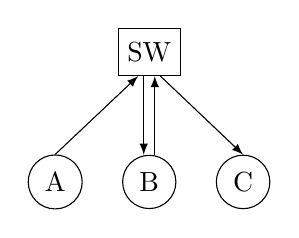
\begin{tikzpicture}[
        server/.style={rectangle, draw=black, fill=white, minimum size=0.6cm},
        switch/.style={rectangle, draw=black, fill=white},
        vm/.style={circle, draw=black, fill=white, node distance=10mm and 5mm},
    ]
    
    \node[server]      	(S1)           				{SW};
    \node[vm]      	   	(V1)         [below=of S1]  {B};
    \node[vm]			(V2)		 [left=of V1]	{A};
    \node[vm]			(V3)		 [right=of V1]  {C};
    
    \draw[-latex] ([xshift=2pt] V1.north) -- ([xshift=2pt] S1.south);
    \draw[-latex] (V2.north) -- ([xshift=-4pt] S1.south);
    
    \draw[-latex] ([xshift=-2pt] S1.south) -- ([xshift=-2pt] V1.north);
    \draw[-latex] ([xshift=4pt] S1.south) -- (V3.north);
\end{tikzpicture}

\end{document}